\documentclass[pdftex,12pt,letter]{article}
\usepackage[margin=0.75in]{geometry}
\usepackage{verbatim}
\usepackage{graphicx}
\usepackage{xspace}
\usepackage{cite}
\usepackage{url}
\usepackage[pdftex,pdfpagelabels,bookmarks,hyperindex,hyperfigures]{hyperref}

\newcommand{\pd}{protoDUNE\xspace}
\newcommand{\pdsp}{pD/SP\xspace}
\newcommand{\xrd}{XRootD\xspace}

\title{The clustered storage option for the protoDUNE NP04 Online Buffer}
\date{\today}
\author{N. Benekos, M. Potekhin and B. Viren}


\begin{document}
\maketitle

\begin{abstract}
\noindent  This note describes the clustered storage
solution for the online buffer for the CERN experiment NP04 which include the single-phase protoDUNE LArTPC detector (\pdsp).
Basic data characteristics and  parameters of such storage are estimated. \xrd is proposed as the underlying
storage clustering technology. It is suggested that a portion of the existing   \textit{Neutrino Platform}
computer cluster at CERN (``neut'') be utilized for the development, testing and actual implementation of the NP04 online buffer. 
\end{abstract}

%%%%%%%%%%%%%
\section{Overview}
\subsection{The Role of the Online Buffer}
\label{sec:the_role}
The online buffer of the NP04 experiment must be put in place to absorb the high instantaneous (in-spill) DAQ
data rate before transmission of raw data to mass storage. It is also needed to satisfy the nominal CERN requirement of
providing 3 days worth of storage to make operation of the experiment possible in case of a network and/or central services
outage. Combined with the projected data rate, this requirement determines the overall capacity of the buffer. From the buffer,
the data needs to be delivered to the high-performance  disk storage (EOS) located at the CERN central services.
The place of the buffer in the data transmission chain therefore can be visualized as in Fig.\,\ref{fig:big-picture}.
EOS serves as the staging area for data transfer to other mass storage facilities such as dCache and tape at FNAL.
\begin{figure}[tbh]
  \centering
  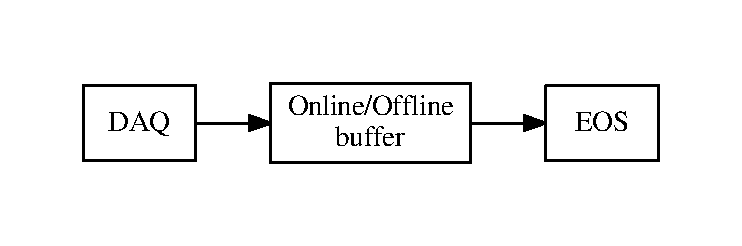
\includegraphics[width=0.7\textwidth]{figures/big-picture.pdf}
  \caption{Place of the buffer in the data transmission chain for NP04.}
  \label{fig:big-picture}
\end{figure}

\subsection{Data Characteristics}

Current estimates \cite{docdb1086} for data rate and volume bracket a range expected
in NP04 \cite{docdb186} when considering in-spill beam triggers and out-of-spill cosmic ray muon triggers.
Three scenarios are considered.  The two that bracket the range are named ``Central'' and ``High rate''.  
Critical assumptions are listed below:
\begin{itemize}
\item beam spill is 4.5 seconds and cycle is 22.5 seconds
\item the beam trigger rate (assumed 25 or 50 Hz)
\item one out-of-spill cosmic trigger for every in-spill beam trigger
\item read out all APAs
\item a compression factor of 4 will be applied in the DAQ
\end{itemize}

\noindent Below is the summary of the principal data characteristics for NP04 at the two ends of their estimated range:

\begin{table}[tbh]
\centering
\begin{tabular}{l l}
\hline
\textbf{Metric} & \textbf{Value} \\
\hline
\hline
trigger rate            & 25 -- 50 Hz \\  \hline
peak data rate          & 1.5 -- 3.0 GB/s \\ \hline
daily data volume       &  25 -- 50TB \\ \hline
3-day buffer capacity   & 150 -- 300TB \\  \hline
\hline
\end{tabular}
\caption{\label{tab:data_char}Expected NP04 data characteristics.}
\end{table}

\subsection{F-FTS}
Basic requirements for the buffer system to handle the NP04 raw data are presented in \cite{docdb1209}.
The design which meets these requirements is outlined in \cite{docdb1212}. It leverages the
Fermi File Transfer System (F-FTS) to manage two essential transfers:
\begin{itemize}
\item from the online buffer to CERN mass disk storage (EOS)
\item from EOS to CERN tape (CASTOR) and  mass storage at FNAL and other US sites
\end{itemize}

\noindent It is foreseen that two distinct instances of F-FTS will be deployed to fill each
respective role. This is schematically illustrated in Fig.\,\ref{fig:ftsinstances} where these instances are labeled ``FTS-1'' and ``FTS-2''.
The ``SP Disk Buffer Farm'' in this diagram corresponds to the NP04 online buffer.

\begin{figure}[tbh]
  \centering
  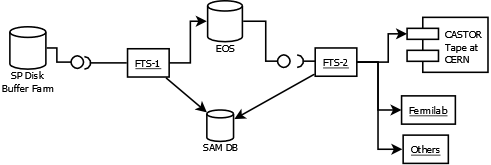
\includegraphics[width=0.7\textwidth]{figures/ftsinstances_v2.png}
  \caption{The two instances of FTS used for marshaling raw data from NP04.}
  \label{fig:ftsinstances}
\end{figure}

F-FTS uses the Fermilab SAM system for file catalog and metadata functionality,
and to keep track of the state of each transfer. In order to make use of this functionality, metadata
needs to be created before F-FTS takes ownership of a particular file. 
Included in this metadata is a file checksum to be used to identify any corruption during file transfer.
We seek to implement a method to calculate the checksum and collect other metadata which does 
not incur an additional read of the file from the buffer storage.

We expect F-FTS to learn of new files in the buffer in one of two
possible modes.  
%
The first option is that we will rely on the ``dropbox'' mode of
operation, whereby F-FTS detects the arrival of a new file according
to configurable rules (e.g. file name patterns). In this mode, F-FTS
must have the ability to list POSIX-like file system directories.
This required functionality would be provided by \xrd's FUSE
interface.
%
The second option is to arrange for F-FTS to be triggered via a HTTP
POST request by an external agent, itself run in response to a trigger
from \xrd signaling the closing of a file.

Independent from the notification mechanism, F-FTS will be responsible
for initiating the transfer of the newly buffered file from the buffer
storage to EOS.  We expect this to be done using F-FTS ``third party
transfer'' mode, specifically by invoking \xrd's direct
server-to-server transfer mechanism (eg \texttt{xrdcp --tpc}).  It is
worth noting that this transfer mechanism does not require exposing
the details of the buffer system.  All file identifiers are in a
common ``\texttt{root://}'' namespace using the host name of the
buffer system \xrd redirector.

\section{Design of the Online Buffer}
\subsection{DAQ Assumptions}
The buffer system design assumes a few high level design features for the DAQ.
The Liquid Argon TPC  and a photon detector subsystem in \pdsp are read out by means of
computing elements (\textit{artDAQ} nodes) called ``Board Readers'' (BR). 
Each reader gets data from a portion of the detector,
and each triggered event must be assembled separately from fragments of the data. This function
is performed by the ``Event Builders'' (EB) nodes, as schematically shown in Fig.\,\ref{fig:upstream}.

\begin{figure}[tbh]
  \centering
  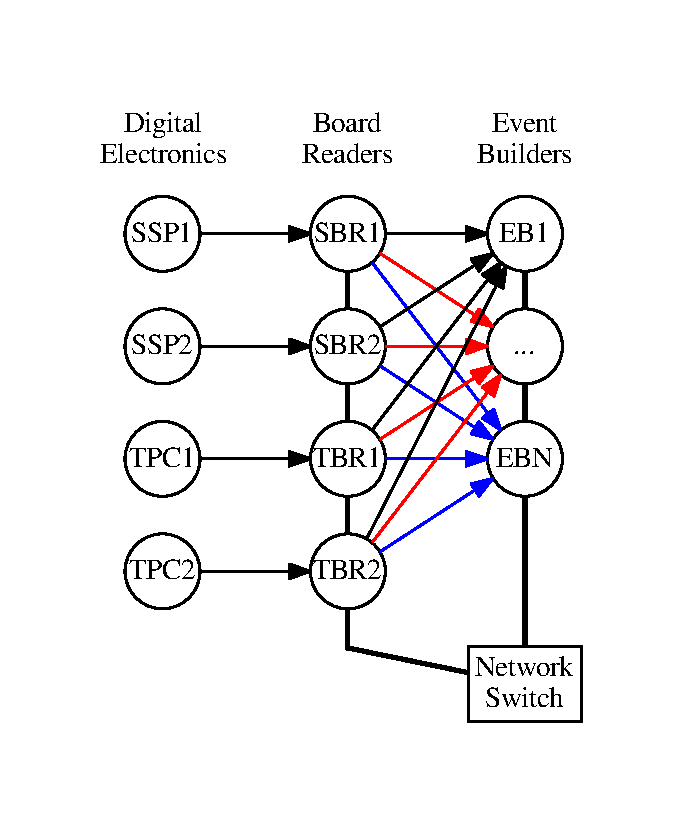
\includegraphics[width=0.5\textwidth]{figures/upstream.pdf}
  \caption{Conceptual diagram of the data flow within DAQ, from the detector to the Event Builders.}
  \label{fig:upstream}
\end{figure}

We assume the routing of data from the BR to the EB layers follows a deterministic round-robin strategy.
We have heard other more sophisticated, less deterministic strategies suggested.


As the name suggests,
the Event Builders create a complete record in memory out of all fragments from the detector for a given trigger (readout period),
which then must be persisted in storage. It is optimal that  this storage also serves as the online buffer 
 which needs to be a part of the system in any case (\ref{sec:the_role}), since otherwise an additional transfer procedure
to a different storage device would need to be implemented and managed.

\subsection{Attached vs Clustered Storage}
Any data taking scenario currently under consideration requires sustained rate
of ``data to disk'' in hundreds of MB per second. In practice this means that
multiple hard drives are needed to absorb such rate and have enough headroom
for stable operation of the system.
There are a few principal options for the placement of storage in the system:
\begin{itemize}
\item SAN (block-level network storage)
\item HDDs attached direectly to each of the Event Builders
\item File-level clustered storage
\end{itemize}

\noindent The SAN option has investigated and rejected for a number of reasons such as difficulty of sharing among multiple
nodes, potential for network bottlenecks etc. The attached storage option is more attractive because of its simplicity and because it
naturally leverages the parallelism of multiple Event Builders.
% and offers transparency for the DAQ developers since it is just a local file system.
However, it also has disadvantages:
\begin{itemize}
\item The transfer agents (F-FTS in the current design) will need to run on each and every EB node. The additional load
due to these processes will depend on the content of the metadata which needs to be produced before the
transfer is actuated, and methods of its gathering (e.g. whether external run conditions database needs to be queried etc).

\item Storage space would be effectively split among individual nodes which could make management of the buffer more difficult.
\end{itemize}

\noindent The file-level clustered storage such as based on \xrd \cite{xrootd} does require additional nodes thus increasing the cost of the system.
At the same time, it offers the following advantages
\begin{itemize}
\item Storage is exposed to its clients as an integral entity as opposed to a number of separate HDDs, and sharing of files over the network
becomes trivial. Integration with ROOT may provide additional convenience to the developers.

\item It provides additional ways to balance the load on the disk drives.

\item Functions related to creation of metadata, checksum etc can now reside in the storage cluster, thus reducing
the load on the Event Builders.

\item Certain features of \xrd  greatly facilitate application development, for example callbacks can be created for various
file operations which is very useful for integration with FTS and other components of the data handling system.
\end{itemize}

\noindent Interaction of the Event Builders with a \xrd storage cluster is schematically shown in Fig.\,\ref{fig:doob-join}.

\begin{figure}[tbh]
  \centering
  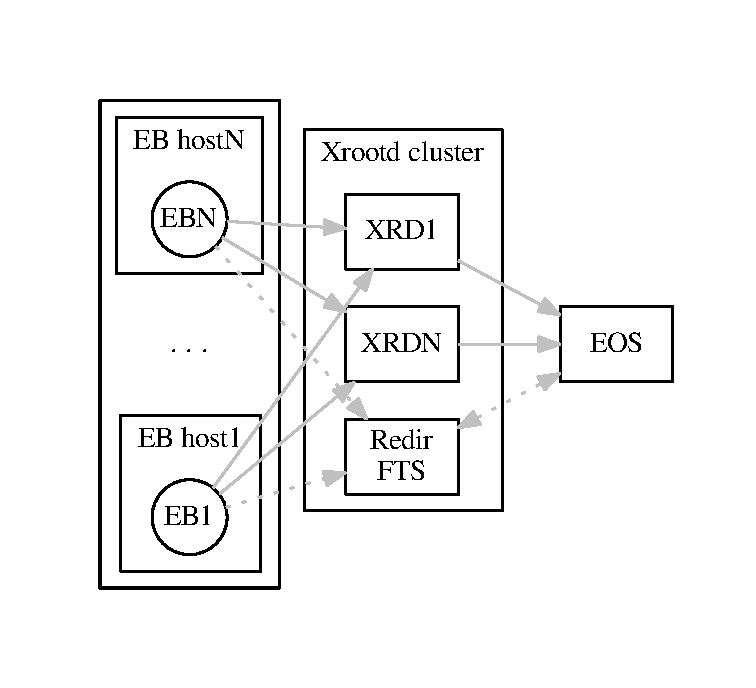
\includegraphics[width=0.5\textwidth]{figures/doob-join.pdf}
  \caption{Conceptual diagram of the Event Builders interfacing the XRootD cluster.}
  \label{fig:doob-join}
\end{figure}

\section{The Cluster}
\subsection{The nodes}

The \textit{CERN Neutrino Platform} cluster (called \texttt{neut}) is now being formed using about 350 nodes in
total reclaimed from ATLAS.  We propose tol dedicate about 50 nodes in
support of developing the online buffer system for the Single-Phase
protoDUNE detector adequately scaled for storing three days worth of
expected data.To label this sub-cluster we will use the name ``\texttt{neut-spbuf}''.

Initially \texttt{neut-spbuf} will be for developing and functional testing of the buffer system design. 
Meanwhile, we will explore what is needed to migrate \texttt{neut-spbuf} into actual
operation and after potential upgrades will proceed to perform scalability testing with realistic data load.

\subsection{The Servers}

The servers in the current \texttt{neut} cluster have very limited disk storage.  The
\texttt{neut-spbuf} nodes must be upgraded to provide storage to meet
the 3-day buffer requirement. To meet the ``High rate'' requirement we
will install $2\times 3$TB SATA disks in each of the 50
\texttt{neut-spbuf} nodes.

On the other hand, each machine has 16\,GB of RAM and right cores running at 2.6\,GHz clock speed,
which makes this a capable computing resource.

\subsection{Networking}

The ``High rate'' scenario requires sinking a peak of 3.0 GByte/sec
(24 Gbps) throughput during the beam spill.  Between spills, when
cosmic muon triggers are acquired, the throughput is somewhat reduced
but we take 3.0 GByte/sec as our requirement.  Spread across the 50
\texttt{neut-spbuf} nodes these streams this will approximately fill
50\% of the existing 1Gbps NICs.  We expect similar multiplicity at
the data production end (the Event Builder layer of the NP04 DAQ).

During initial testing we will request a 20 Gbps link between the
current location of \texttt{neut}\footnote{CERN building 185} and
central CERN computing services including EOS and the NP04 detector
site\footnote{CERN building EHN1}.

To supply this connectivity we require 50 switch ports at 1Gbps and
(effectively) one switch port at 20Gbps.  Based on our current design
it is possible to segment the network streams so that the total
bandwidth is spread over multiple switches, for example two switches
each with 25 ports at 1Gbps and 1 port with 10 Gbps.  One example
switch is the Cisco SG500X-48P which can provide 48 1Gbps ports and
ample ports on the high-bandwidth side.  One such switch is needed on
the DAQ end of the 20Gbps link and one on the \texttt{neut-spbuf} end.

\section{Additional Work Items}
A few items will require additional R\&D, such as
\begin{itemize}
\item Where the metadata will be produced, e.g. in the Event Builders or on the machines
in the \texttt{neut} cluster
\item What is the exact mechanism of interaction between the \xrd middleware and the FTS; our initial intention
is to use HTTP notification of FTS which is in turn activated by the \xrd ``ofs.hotify'' mechanism. Generation
of the necessary metadata will also need to be activated at this point in the data path, and the necessary software
is yet to be designed.
\end{itemize}



\begin{thebibliography}{1}
\bibitem{docdb1086}
{DUNE DocDB 1086: \textit{ protoDUNE/SP data scenarios with full stream (spreadsheet)}}\\
\url{http://docs.dunescience.org:8080/cgi-bin/ShowDocument?docid=1086}

\bibitem{docdb186}
{DUNE DocDB 186: \textit{ ProtoDUNE Proposal}}\\
\url{http://docs.dunescience.org:8080/cgi-bin/ShowDocument?docid=186}


\bibitem{docdb1209}
{DUNE DocDB 1209: \textit{Basic Requirements for the protoDUNE Raw Data Mangement System}}\\
\url{http://docs.dunescience.org:8080/cgi-bin/ShowDocument?docid=1209}


\bibitem{docdb1212}
{DUNE DocDB 1212: \textit{Design of the Data Management System for the protoDUNE Experiment}}\\
\url{http://docs.dunescience.org:8080/cgi-bin/ShowDocument?docid=1212}



\bibitem{xrootd}
{XRootD, high performance, scalable fault tolerant access to data  repositories}.\\
  \url{http://xrootd.org/}.

\end{thebibliography}


\end{document}

%%% Local Variables:
%%% mode: latex
%%% TeX-master: t
%%% End:
